\section{Appendix}
\subsection{Diagrams}

\begin{figure}[H]
    \centering
    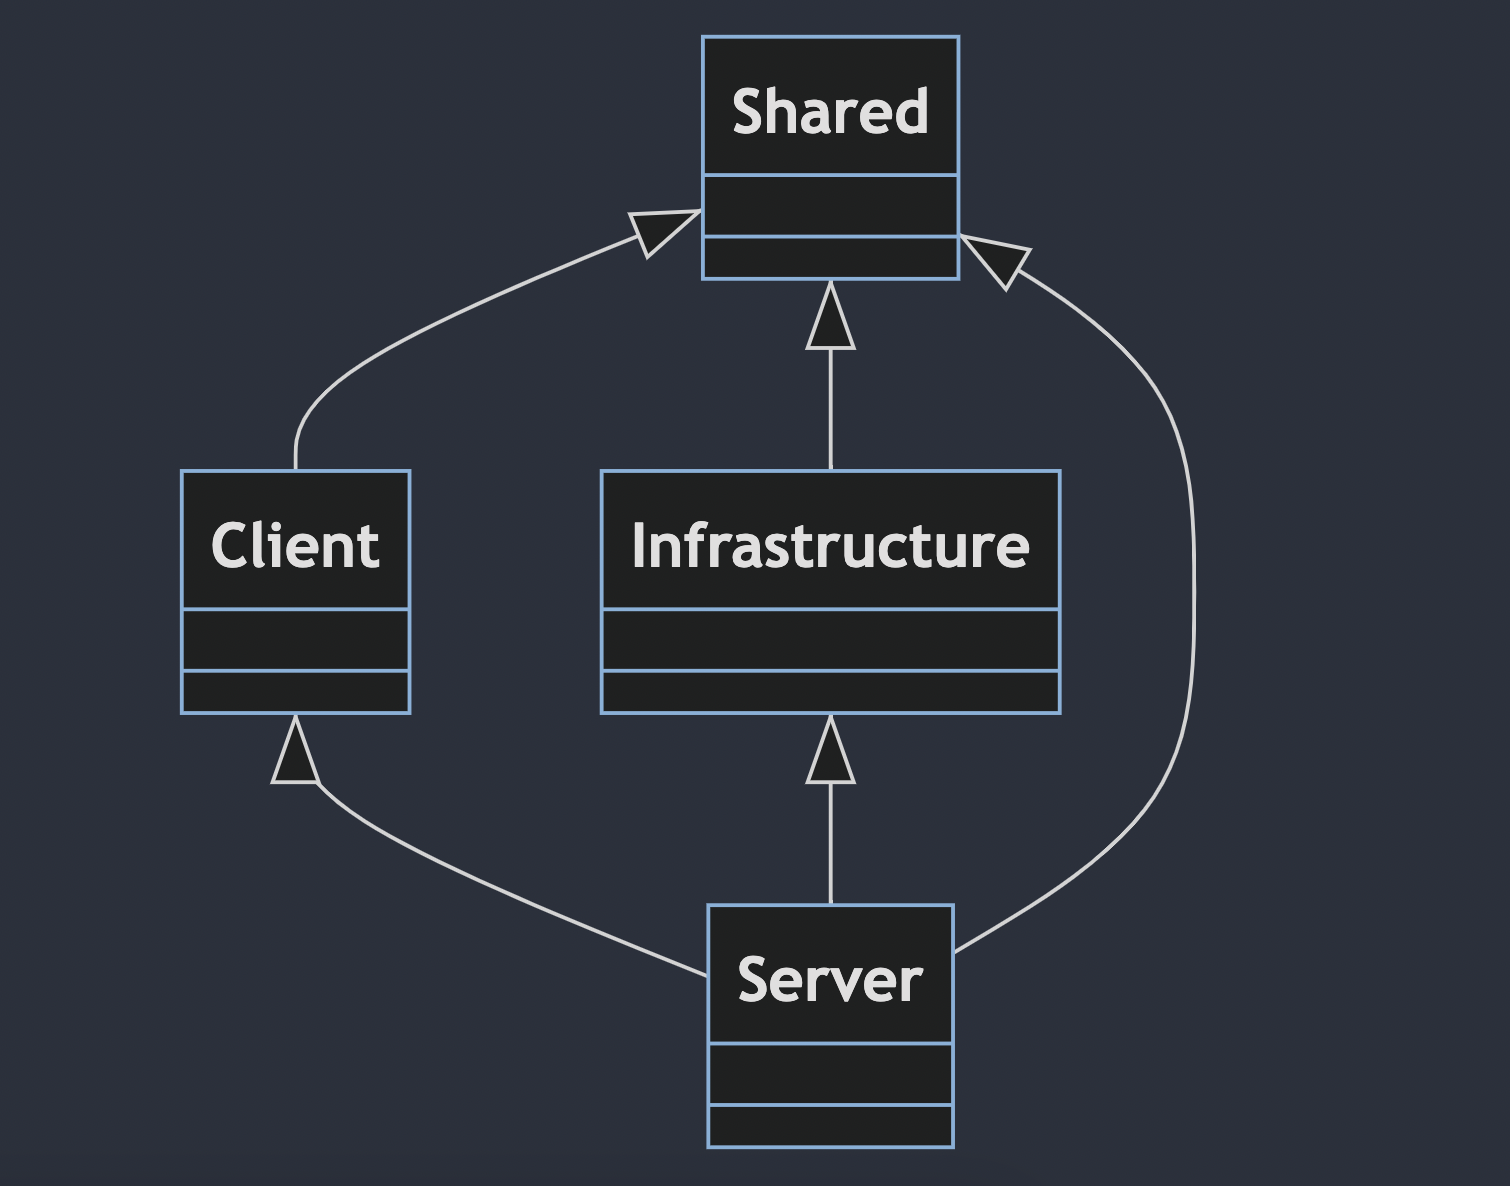
\includegraphics[width = 15.0cm, height = 8.0cm]{Images/onionStructure.png}
    \caption{Larger version of the project dependency graph}
    \label{fig:LargerProjectDependencyGraph}
\end{figure}

\begin{figure}[H]
    \centering
    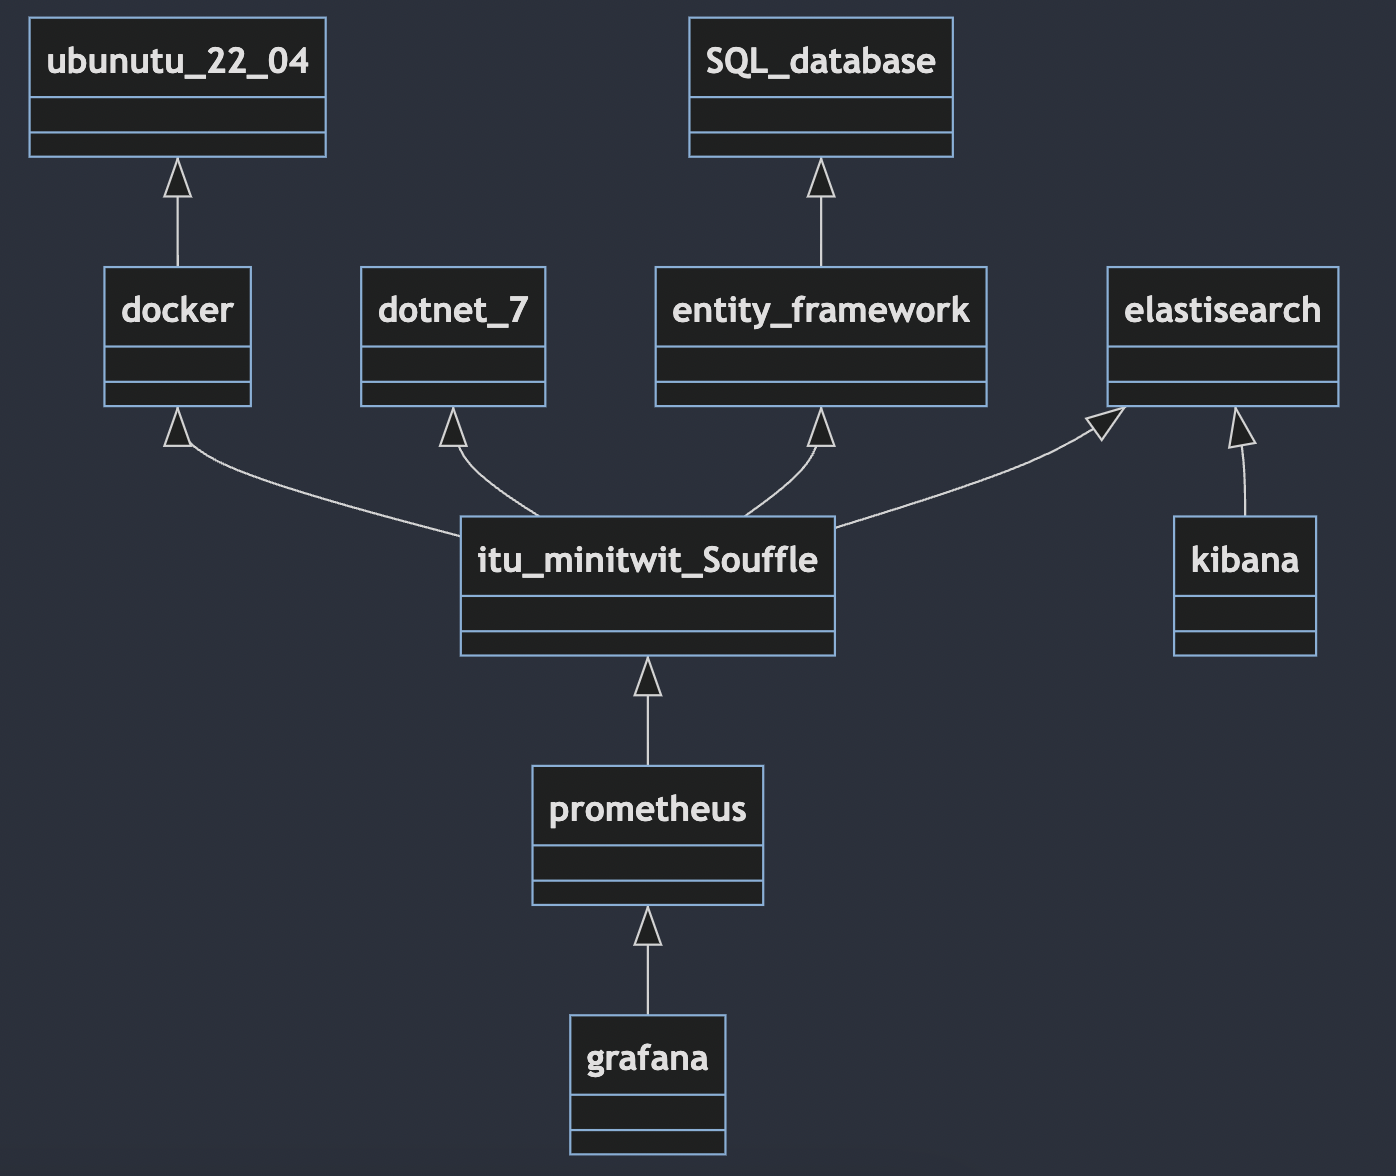
\includegraphics[width = 15.0cm, height = 12.0cm]{Images/application_dependencies.png}
    \caption{Larger version of the application dependency graph}
    \label{fig:LargerApplicationDependencyGraph}
\end{figure}

\begin{figure}[H]
    \centering
    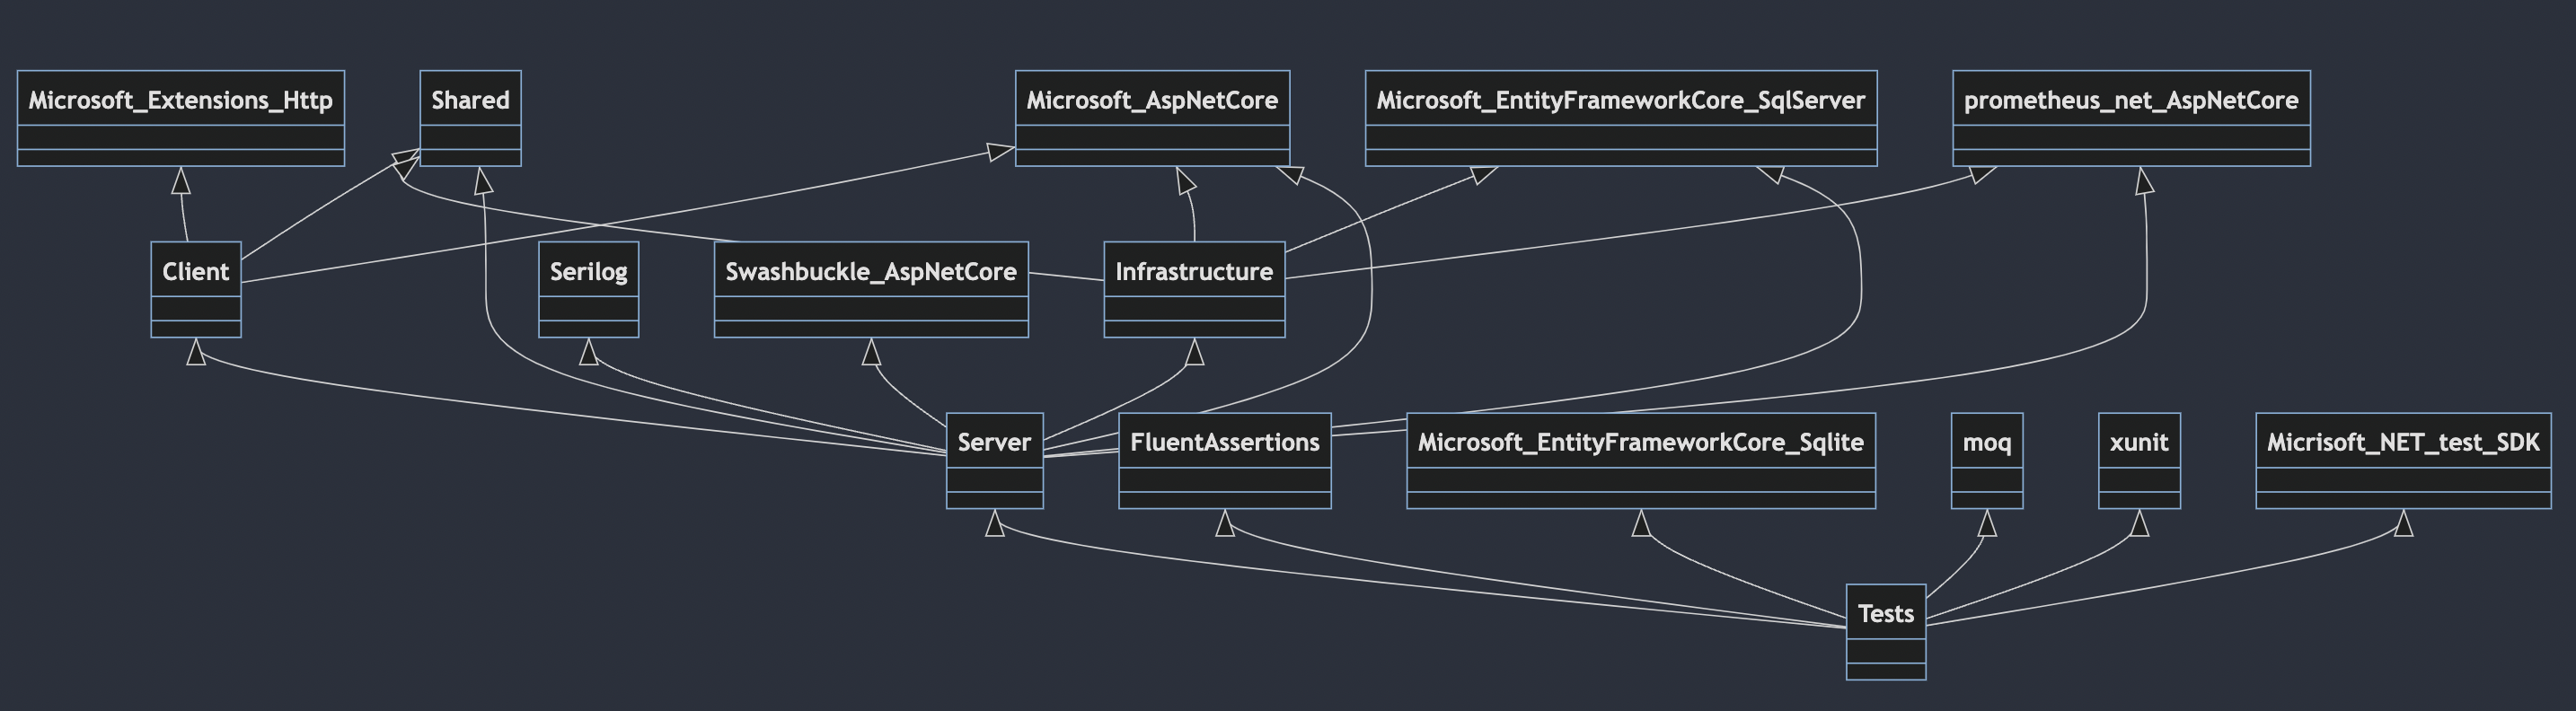
\includegraphics[angle = 90, width = 300pt, height = 700pt]{Images/dependencies2.png}
    \caption{Larger version of Package dependency graph for C\# application}
    \label{fig:packageDependencyGraph2}
    \centering
\end{figure}

\begin{figure}[H]
    \centering
    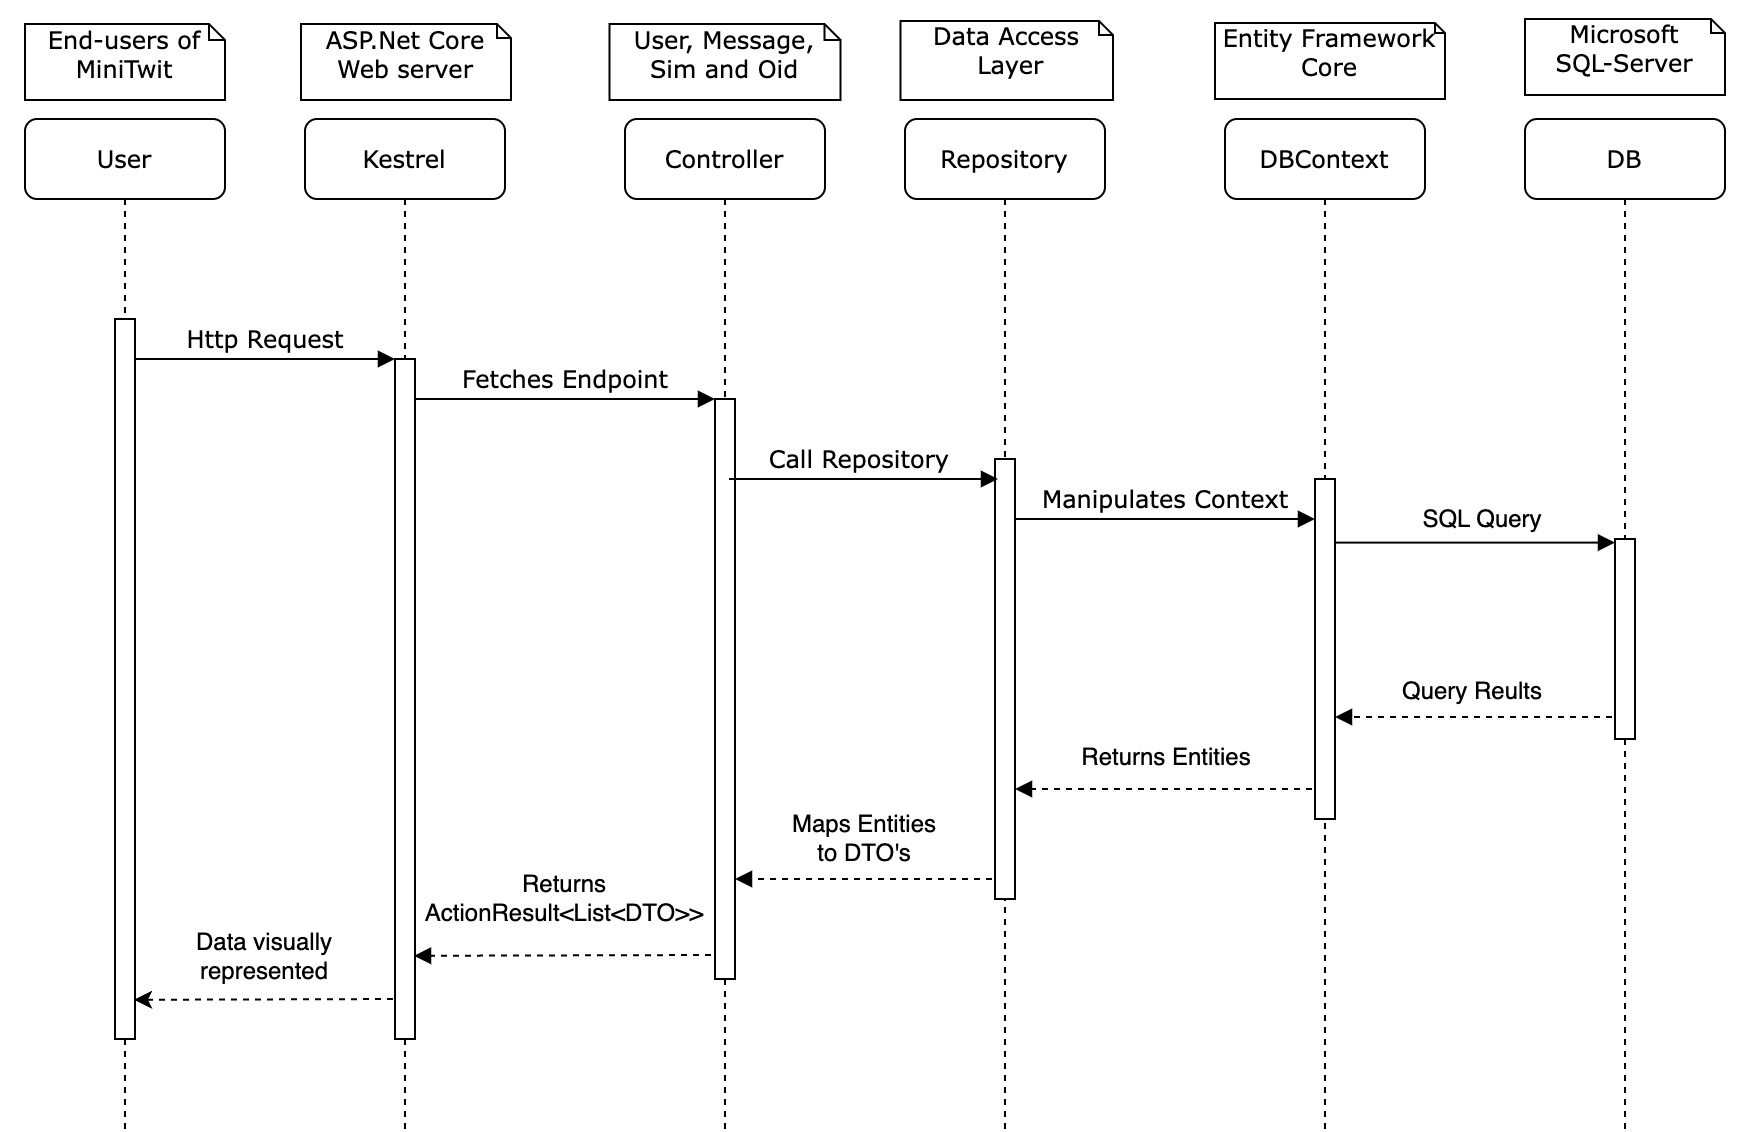
\includegraphics[angle=90, width=15.0cm]
    {Images/SequenceDevOps.jpg} 
    \caption{Larger version of API sequence diagram}
    \label{fig: Vertical Data Journey}
\end{figure}
\newpage

\begin{figure}[H]
    \centering
    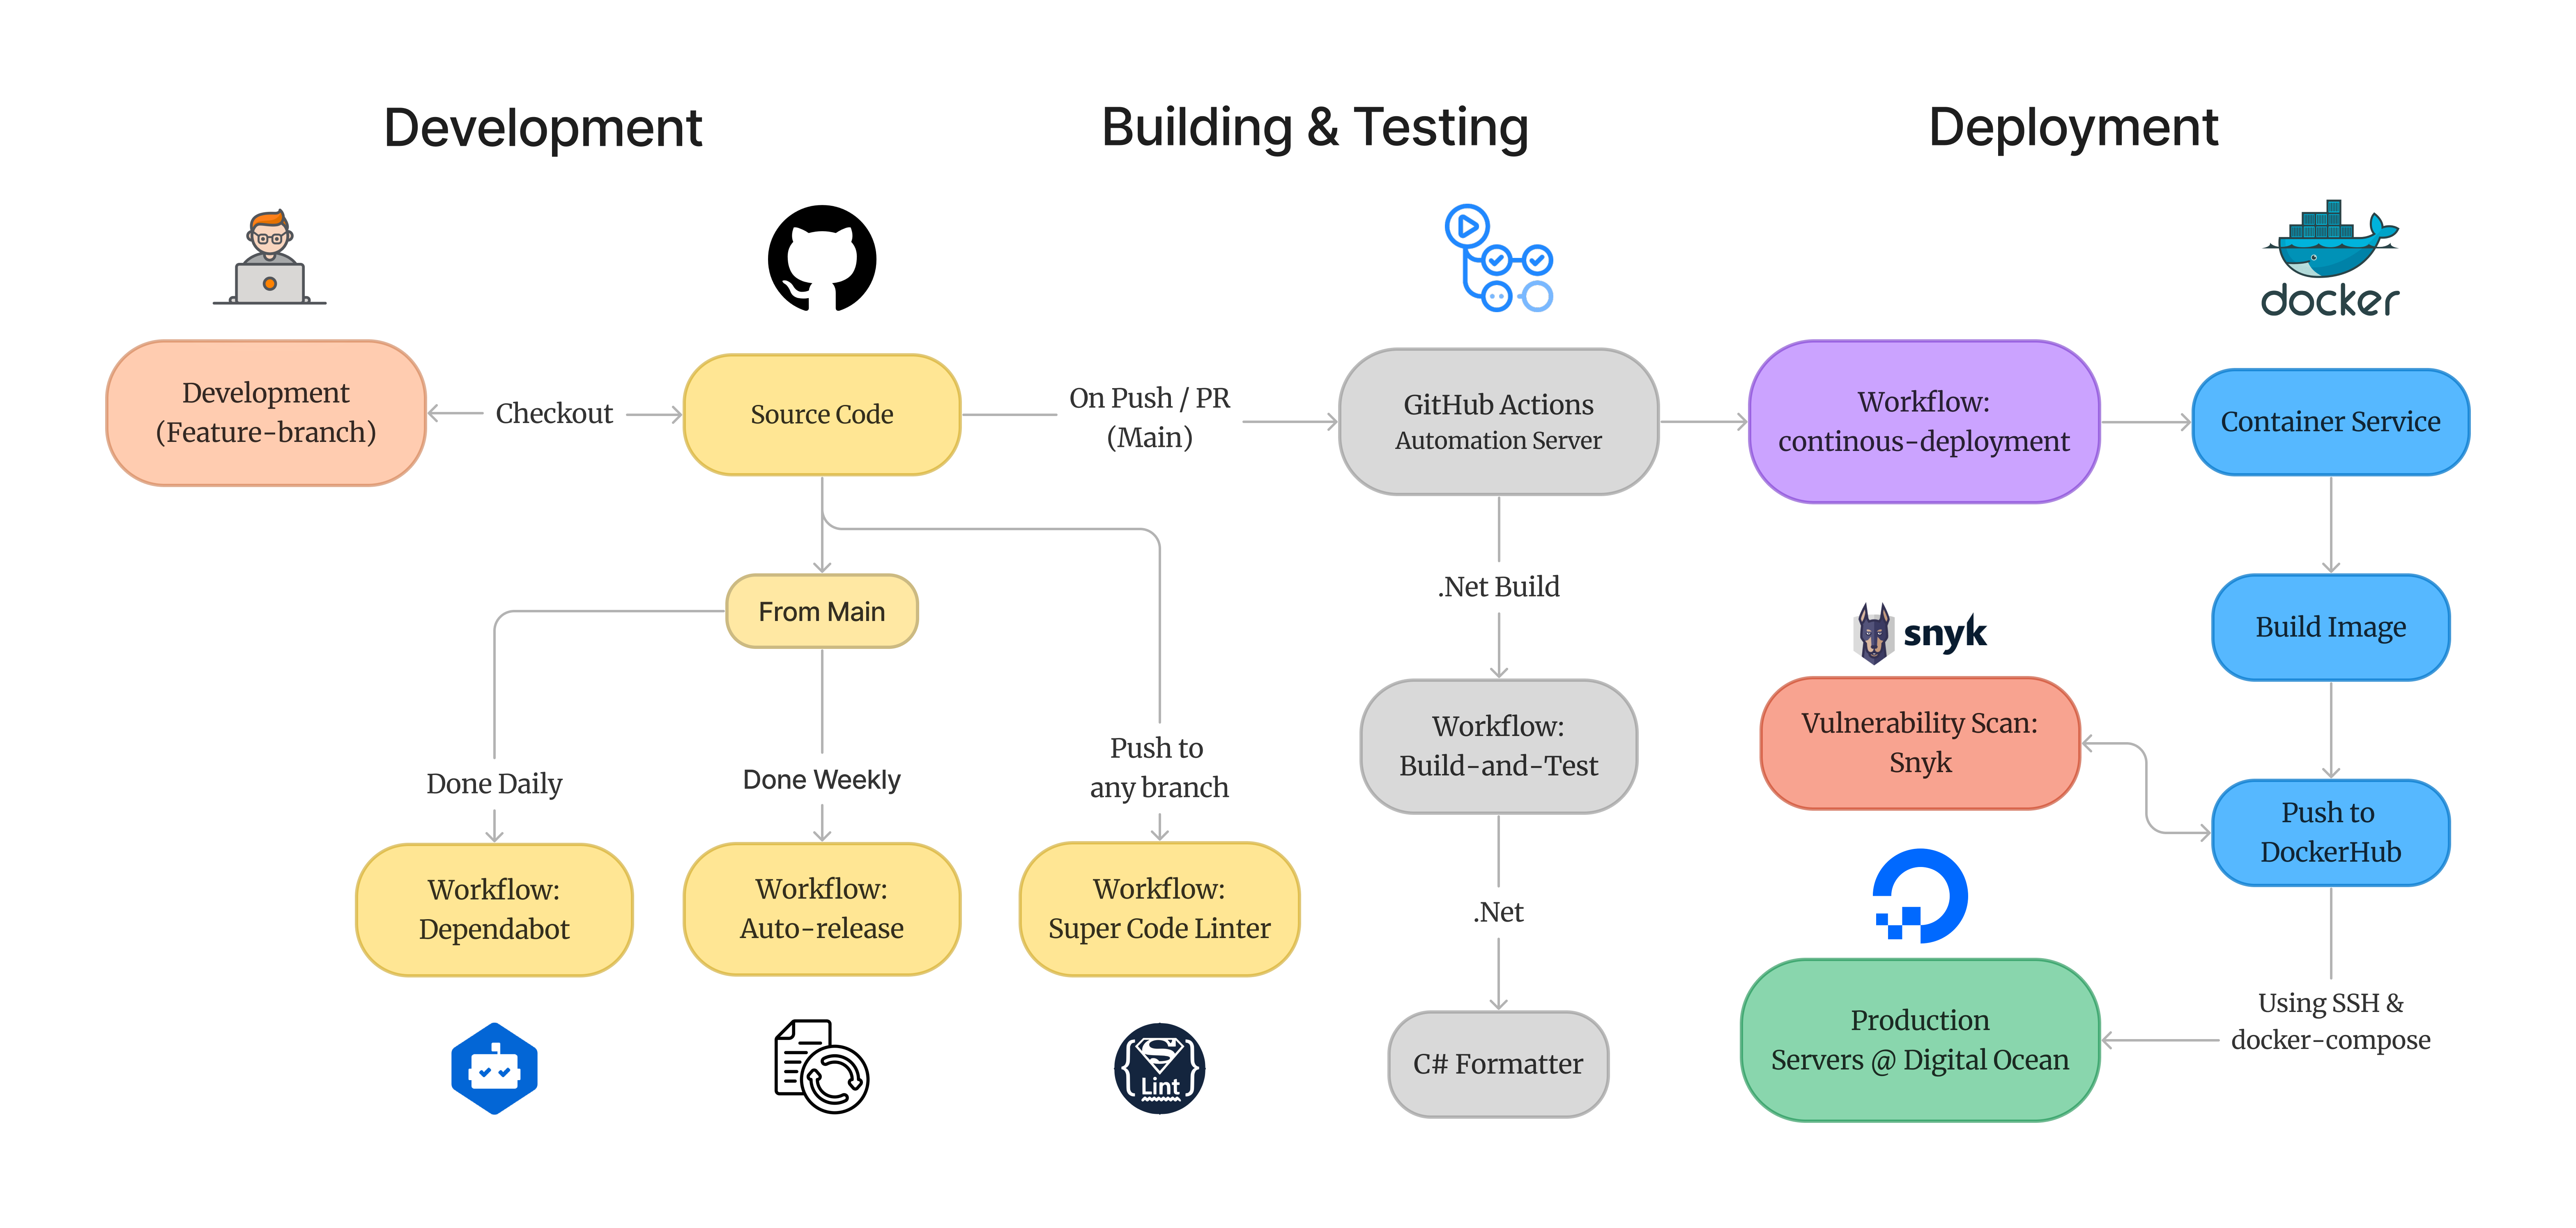
\includegraphics[angle=90, height=720pt]{Report/Images/CICD_Chain.png} 
    \caption{Larger version of CI/CD tech-stack}
    \label{fig:Vertical CI/CD tech-stack}
\end{figure}
\newpage





